\section{Thảo luận và kết luận}
\label{sec:thaoluan}

\subsection{Hạn chế (phải nêu rõ)}
Kết quả \emph{chạy được} không đồng nghĩa với \emph{đáng tin}.

\textbf{H1 --- Nội suy đóng góp một phần (chính sách 3 mức).}
Với scope gộp QN+HP ban đầu, đường 4-feature fail hết $\Rightarrow$ 100\% trung vị. Sau khi \textbf{tách HP-only} $+$ áp \textbf{chính sách 3 mức} $+$ bổ sung Salinity, trạm Cát Bà có \textbf{3 chỉ số ML-grounded}: DO (mạnh, $0{,}535$), Salinity (mạnh, $0{,}673$) $+$ PO4 (yếu, $0{,}233$, có cờ). Kim loại, Coliform, H2S vẫn là trung vị --- đã kiểm định không đoán được (Mục~\ref{sec:median-evidence}).

\textbf{H2 --- Nhãn vẫn lệch về ``phù hợp'' (đã giảm nhờ Salinity).}
Ngày 20/06 TSS và nhiệt độ đều vượt ngưỡng, nhưng nhãn vẫn ``phù hợp'' ($0{,}900$), vì $\sim$71\% đầu vào vẫn là trung vị ``nước khỏe'' nuốt chửng các chỉ số thật. Việc đưa \textbf{Salinity} (chỉ số quan trọng thứ 2) từ hằng số sang model-grounded đã \emph{giảm} mức chi phối của hằng số, nhưng kim loại/Coliform vẫn cố định nên nhãn nối đất còn yếu.

\textbf{H3 --- $R^2\approx0{,}9999$ của BOD5/Alkalinity là artifact.}
Tương quan BOD5--COD $=0{,}977$ và Alkalinity--COD $=0{,}955$ (không có cơ sở hóa học). Hình~\ref{fig:artifact} cho thấy các điểm nằm trên một đường gần như \emph{tất định} --- quan hệ hàm do quá trình sinh dữ liệu, không phải tương quan sinh thái học được. ``Thành công'' của 5-feature phụ thuộc hoàn toàn vào COD --- đúng cảm biến đã chết.

\begin{figure}[h]
\centering
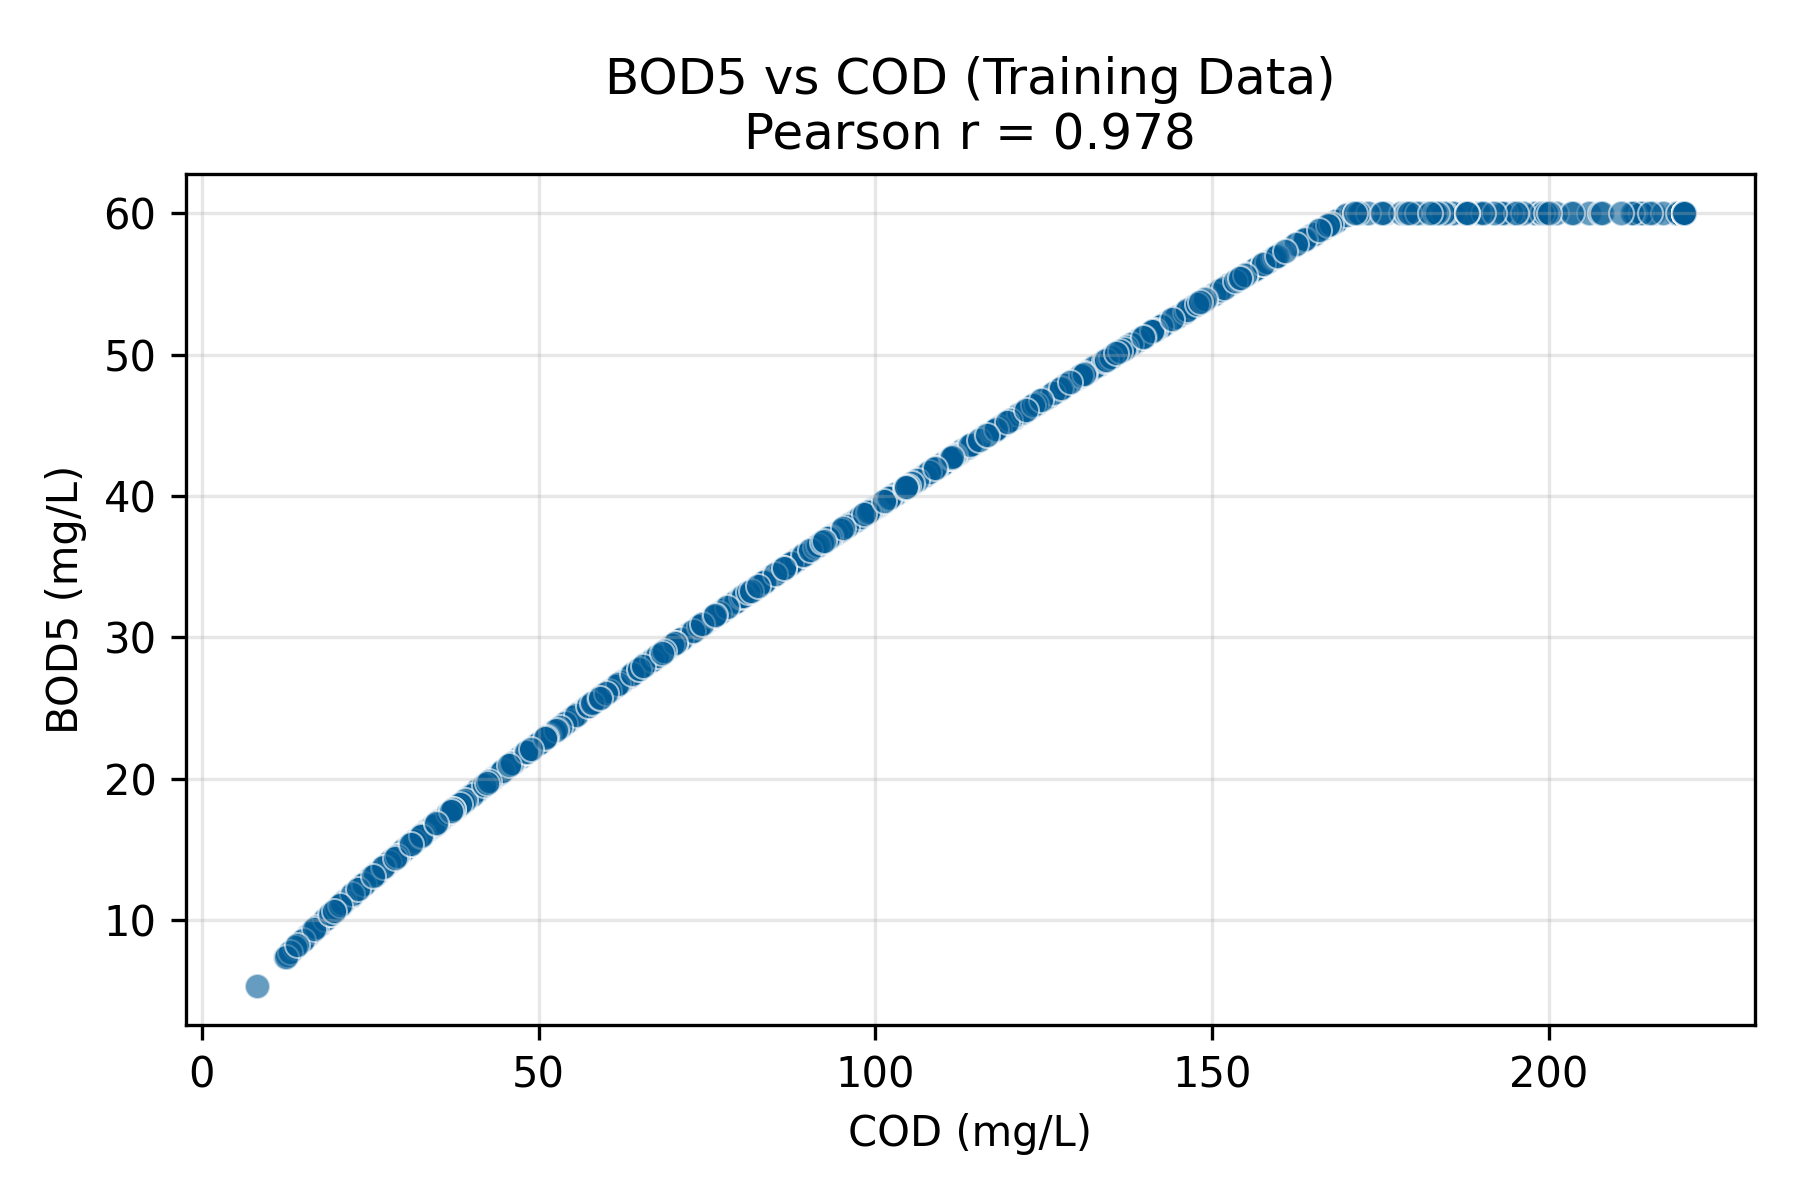
\includegraphics[width=\linewidth]{../figures/bod5_cod_scatter.png}
\caption{BOD5 và Alkalinity trong dữ liệu huấn luyện QN/HP gần như là hàm tất định của COD (điểm bám sát một đường). Đây là lý do $R^2$ chạm 0{,}999 --- artifact của dữ liệu, không phải khả năng dự báo thực.}
\label{fig:artifact}
\end{figure}

\textbf{H4 (đã đính chính) --- DO dự báo được KHI tách đúng vùng.}
Kết luận trước (``DO không đoán được'') là \emph{artifact của scope gộp QN+HP}: trộn hai vịnh khác chế độ làm nhiễu quan hệ. Tách HP-only $\Rightarrow$ DO đạt $R^2=0{,}535$ (Hình~\ref{fig:do}) --- mức vừa nhưng hơn hẳn trung vị. Bài học phương pháp: \emph{chọn sai phạm vi dữ liệu có thể che giấu tín hiệu thật}. Riêng QN, DO vẫn không đoán được ($R^2<0$) --- cần xem lại khi bật trạm Vân Đồn.

\warnbox{\textbf{Khuyến nghị sử dụng:} phần \emph{giám sát QCVN} (5 chỉ số thật) hữu ích và đáng tin. Phần \emph{phân loại} hiện chỉ nên trình bày như \textbf{pipeline demo}, chưa đủ tin cậy để ra quyết định nuôi trồng cho tới khi: (a) bổ sung cảm biến DO + độ muối, (b) sửa cảm biến COD, (c) xác nhận đơn vị NH4.}

\subsection{Kết luận và hướng phát triển}
Module \texttt{lab/realtime\_greenlab/} đã thiết lập đầy đủ đường ống từ MongoDB thời gian thực tới nhãn phù hợp, kèm kiểm soát chất lượng cảm biến, quy đổi hóa học NH3, và nội suy thích nghi theo vùng --- toàn bộ kèm cảnh báo xuất xứ minh bạch. Quá trình cho thấy hai bài học phương pháp: (1) \emph{kiểm tra dữ liệu trước khi tin mô hình} (phát hiện COD chết); (2) \emph{phạm vi dữ liệu huấn luyện quyết định kết quả} (tách HP-only cứu tín hiệu DO mà scope gộp đã che giấu). Đây là kết quả khoa học trung thực, đáng nêu trong luận văn hơn một con số ``phù hợp'' đẹp nhưng rỗng.

\textbf{Hướng phát triển:}
\begin{enumerate}[nosep]
  \item Kích hoạt thu thập trạm Vân Đồn (QN) để mở rộng sang oyster.
  \item Bổ sung cảm biến DO + độ muối --- hai chỉ số hiện đang là hằng số.
  \item Xác nhận đơn vị NH4 với nhà cung cấp; cập nhật \texttt{NH4\_UNIT\_SCALE}.
  \item Khi đủ chuỗi thời gian, thử dự báo (forecast) chỉ số tương lai thay vì chỉ phân loại tức thời.
  \item Tích hợp phần giám sát QCVN (đã đáng tin) vào webapp.
\end{enumerate}
